\chapter{Acquisition-System Design}
\section{Overview}
This section covers the development process including the hardware and firmware design of the audio acquisition system.
The goal of the acquisition system is to provide a flexible microphone recording infrastructure to easily aquiring audio signals from multiple microphones.


\subsection{Key Requirements}
% The main focus of the development is to design a professional looking, easy to use and eye-catching device for demonstration purposes.
% The project name \textit{Audio-Beamformer} has been chosen as it is easy to remember and has potential to be seen as a trademark.

The following key requirements have been set:
% \begin{itemize}
% 	\item Single power adapter or power cable (e.g. no need of labor power supplies)
% 	\item Easy to install (e.g. montage on a camera tripod)
% 	\item Intuitive to operate via state-of-the-art graphical user interface
% 	\item Multiple audio streaming sources such as Bluetooth and USB input devices
% 	\item Great scalability and flexibility of the hardware and software design
% \end{itemize}

\subsection{Key Decisions}



\newpage
\section{Hardware Design}

\begin{figure}[h]
	\centering
	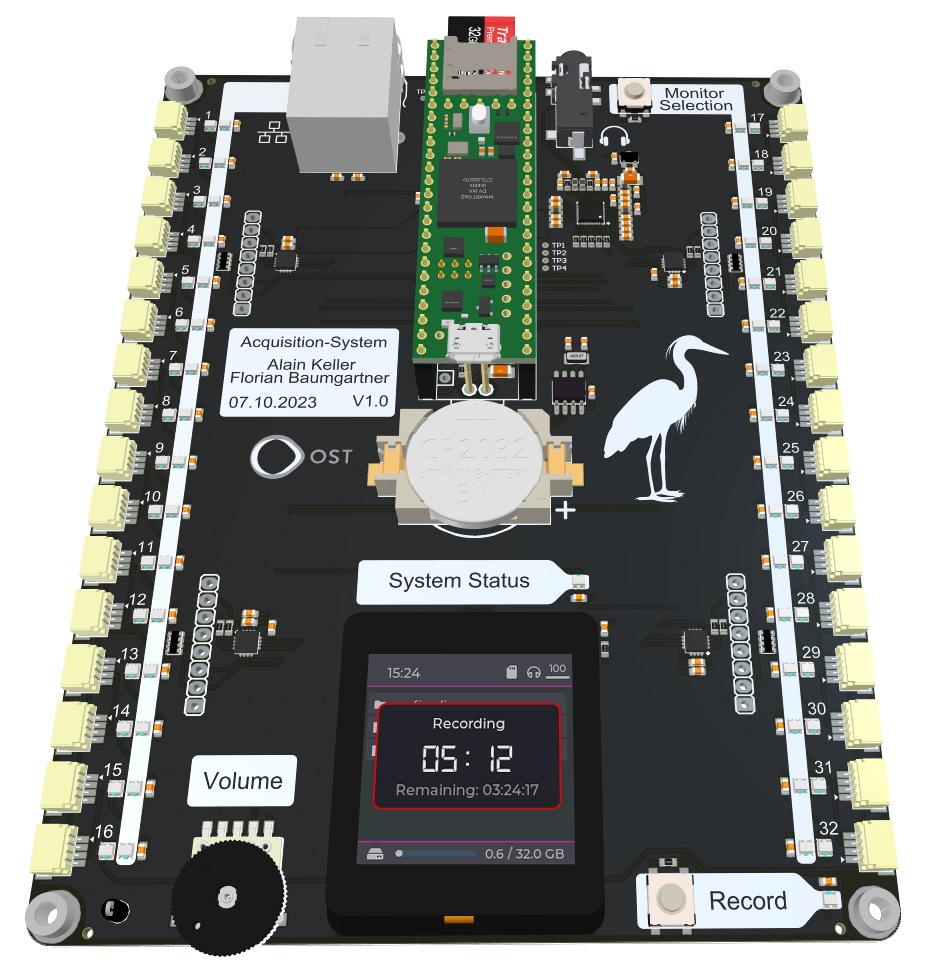
\includegraphics[width=1.0\textwidth]{images/4_design_acquisition_system/Acquisition_System_Front.png}
	\caption{Front view of the Acquisition System}
	\label{fig:acquisition_system_front}
\end{figure}


\subsection{Block Diagram}

\begin{figure}[h]
	\centering
	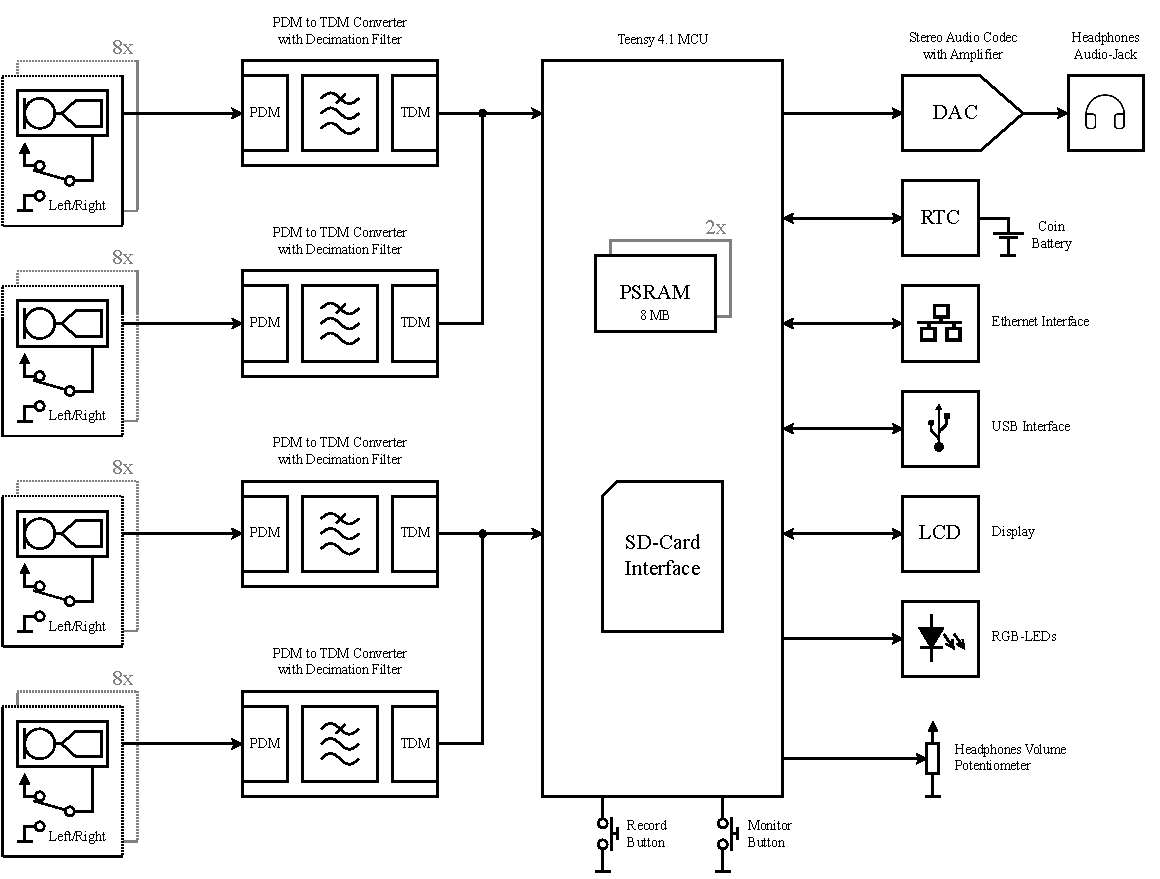
\includegraphics[width=1.0\textwidth]{images/4_design_acquisition_system/system_block_diagram.pdf}
	\caption{System block diagram}
	\label{fig:system_block_diagram}
\end{figure}

\subsection{Microcontroller Unit (MCU)}

%  TODO: Write about external PSRAM


\subsection{Audio Input}

\subsection{Audio Processing}

\subsection{Headphone Output}

To prelisten the individual audio channels, a headphone output is implemented.

% description of headphones jack
The headphone output is a standard 3.5mm stereo jack.



\newpage
\section{Firmware Design}
Blabla

\subsection{Graphical User Interface (GUI)}

\subsection{GUI Pages}

\begin{minipage}{\linewidth}
	\begin{wrapfigure}{l}{4.5cm}
		\vspace{-0.6cm}
		
\includegraphics[width=4cm]{images/4_design_acquisition_system/gui/01_splash_screen.png}
		\centering
		\caption{Splash screen}
		\label{fig:acquisition_system_gui_splash_screen}
	\end{wrapfigure}
	\subsubsection{Splash Screen}
	When the device is powered on, the splash screen is displayed until the boot process is finished.
	On average this takes about 5 seconds.
\end{minipage}
\vspace{-0.2cm}



